\documentclass[10pt,twocolumn,letterpaper]{article}

\usepackage{cvpr}
\usepackage{times}
\usepackage{epsfig}
\usepackage{graphicx}
\usepackage{amsmath}
\usepackage{amssymb}

% Images
\usepackage{graphicx}
\usepackage{float}
\graphicspath{{./images}}

% Include other packages here, before hyperref.
\usepackage[table]{xcolor}

% If you comment hyperref and then uncomment it, you should delete
% egpaper.aux before re-running latex.  (Or just hit 'q' on the first latex
% run, let it finish, and you should be clear).
\usepackage[breaklinks=true,bookmarks=false]{hyperref}

\cvprfinalcopy % *** Uncomment this line for the final submission

\def\cvprPaperID{****} % *** Enter the CVPR Paper ID here
\def\httilde{\mbox{\tt\raisebox{-.5ex}{\symbol{126}}}}
\def\code#1{\texttt{#1}}

% Pages are numbered in submission mode, and unnumbered in camera-ready
%\ifcvprfinal\pagestyle{empty}\fi
\setcounter{page}{1}
\begin{document}

%%%%%%%%% TITLE
\title{Applying Sketch Recognition Techniques to Play Pictionary with a Computer}

%%%%%%%%% AUTHOR
\author{Michael Chen\\
University of Texas at Austin\\
{\tt\small mxchen2001@utexas.edu}
\and
Satya Boddu\\
University of Texas at Austin\\
{\tt\small satyaboddu@utexas.edu}
\and
Ishan Shah\\
University of Texas at Austin\\
{\tt\small ishan0102@utexas.edu}
\and
Rishi Ponnekanti\\
University of Texas at Austin\\
{\tt\small rishiponnekanti@utexas.edu}
\and
Udai Jain\\
University of Texas at Austin\\
{\tt\small udaij12@utexas.edu}
}

\maketitle
%\thispagestyle{empty}

%%%%%%%%% PAPER
%--------------------------------------------------------------------------
{\centering \section*{Abstract}}

\emph{We present an implementation of a neural network that can classify sketch drawings. This model was trained on a dataset of millions of human-drawn images and built into a playable Pictionary game against the computer. We also show an exploration into using Generative Adversarial Networks (GANs) to allow the computer to create sketches.} \vspace{1em}

%--------------------------------------------------------------------------
\section{Introduction}

The fields of sketch recognition and sketch generation have had massive advancements in the past few years due to the onset of neural networks with millions of parameters. These neural networks are able to identify images, text, and more by stacking independent layers of nodes in a way that mimics the structure of the human brain. Our goal with this project was to take these neural networks and apply them to Pictionary, a classic game that involves one person trying to guess another’s drawing.

Developing a model to play Pictionary is uniquely challenging in how the training data differs from natural images. Humans tend to interpret the same objects in dramatically different ways making it hard to create a uniform training set. Additionally, sketches contain less data than images since they are usually black-and-white and have no background information. While these caveats produce challenges, the silver lining is that the lack of data inherently limits the complexity of the training set, making it easier for the model to figure out what makes objects unique.

Lastly, we are interested in having the computer not only predict sketch classes but to also produce sketches. We attempt to use GANs to solve this problem by generating images from random noise until a discriminator cannot tell the difference. We base our work around solving these problems and aim to lay groundwork for making human-computer interaction more tractable.

%--------------------------------------------------------------------------
\section{Related Work}

Sketch recognition and generation have been studied quite extensively, and many datasets exist for both tasks. Unique aspects of sketches such as stroke order, as compared to traditional images, have inspired many different approaches to these tasks. Sketch generation has not seen as much success as recognition, but there have been interesting approaches that involve completing a sketch in a step-by-step fashion.

%--------------------------------------------------------------------------
\subsection{Google Quick, Draw!}

In 2016, Google launched Quick, Draw!, a game allowing users to play Pictionary against a computer. This game involved users drawing a given object and a neural network attempting to guess what they were drawing in real time. The model improved as users played the game through reinforcement learning, where more user data made the model more robust at understanding how to classify sketches. The resulting user drawings were stored in what is known as the Google Quick, Draw! dataset \cite{QuickDraw}, which contains over 50 million drawings spanning 345 categories of sketches. This dataset provides preprocessed sketch data with information about stroke order \cite{QuickDraw}.

\begin{figure}[H]
  \centering
  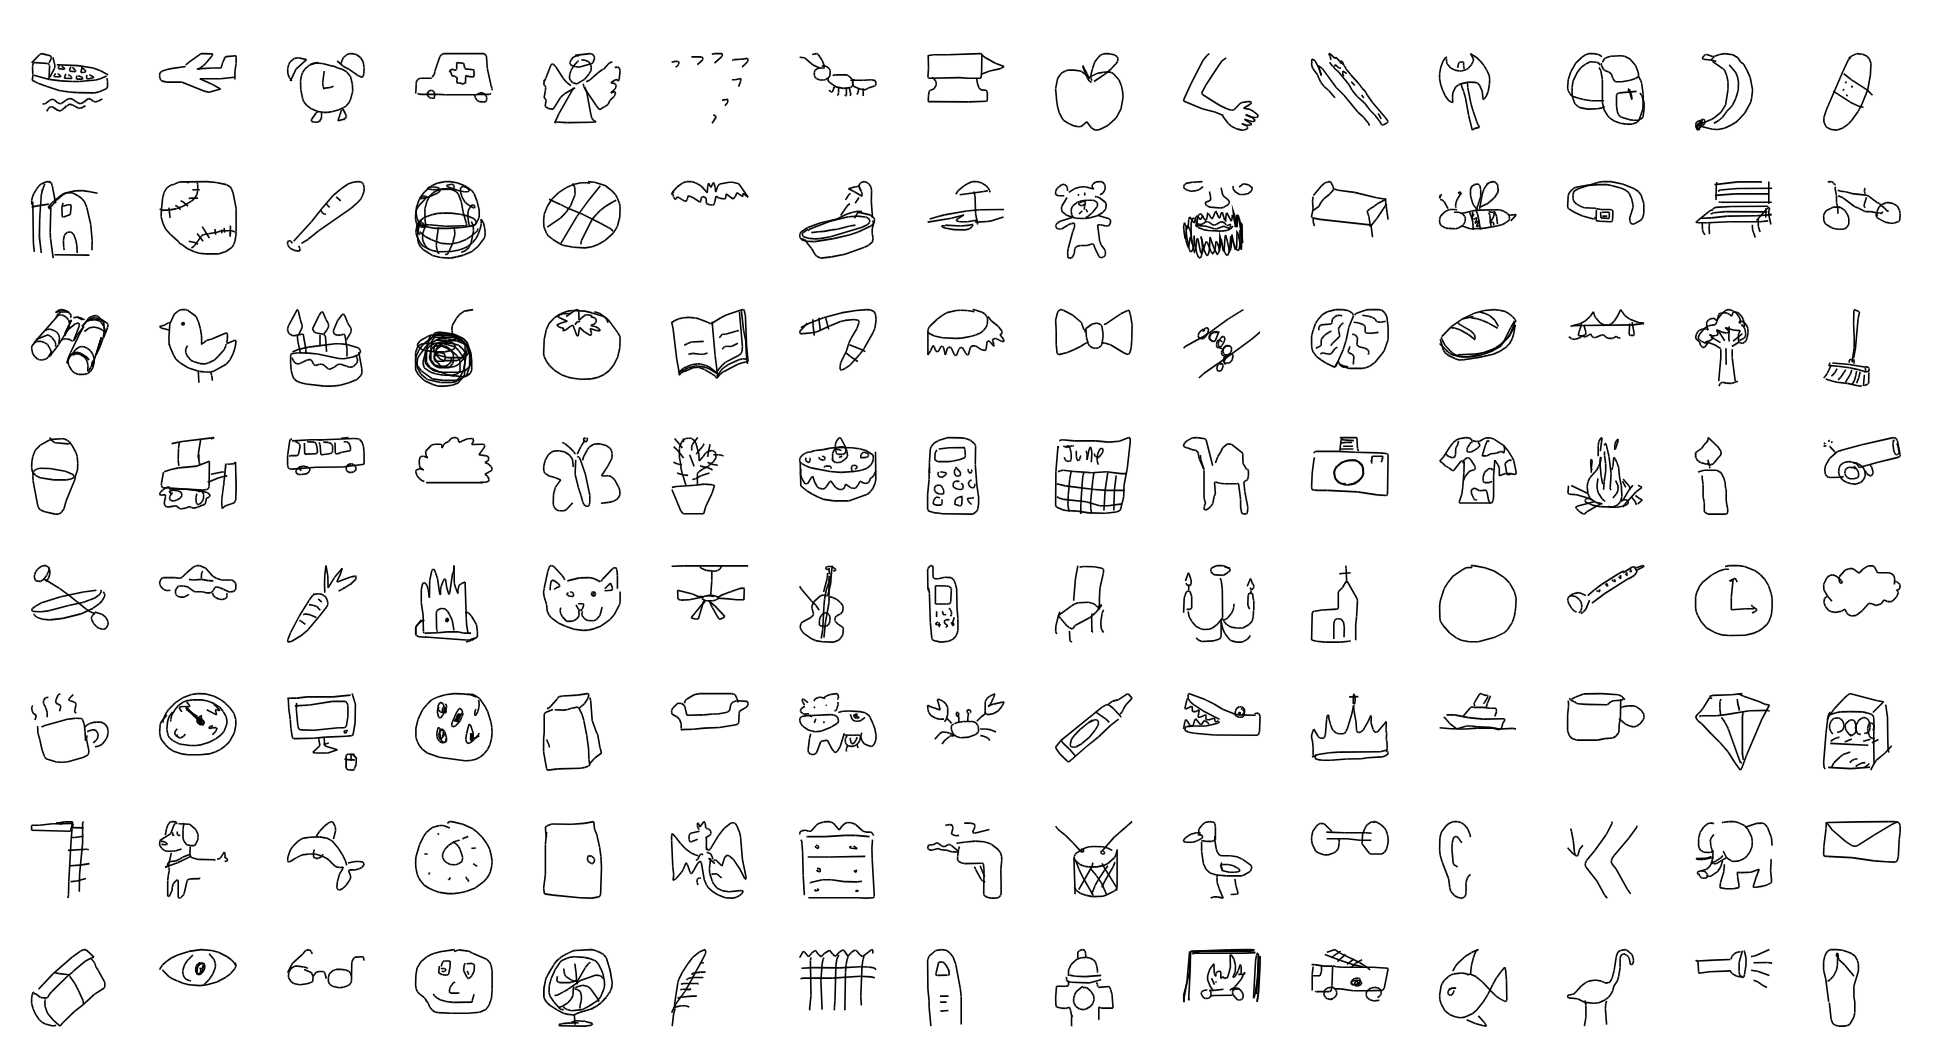
\includegraphics[width=0.45\textwidth]{quickdraw_samples.png}
  \caption{Quick, Draw! Sample Images}
\end{figure}

Many projects have been built atop this dataset, one of which is Google’s own \code{sketch-rnn} model, an RNN designed to construct sketches given an object\cite{sketch-rnn}. This is the opposite of the previous task, as the neural network is now the artist rather than the guesser. We discuss our approach to sketch generation with GANs using Google’s dataset further on. Additionally, we use this dataset to train an RNN that can predict sketch classes. Because this dataset is so expansive, it is extremely useful for a multitude of applications.

%--------------------------------------------------------------------------
\subsection{Sketch Recognition}

There has been significant research to develop models that outperform typical convolutional neural networks (CNNs) and RNNs for sketch generation. One such paper proposes not using training of any kind, and focuses on interpreting diagrammatic sketches \cite{sketchRead}. Another paper discusses the benefits of using a multi-kernel method, which focuses on individual features to determine the classification \cite{LI20151}. Yet another paper introduces a Graph Neural Network called the Multigraph Transformer that is shown to outperform CNNs and RNNs on the Quick, Draw! Dataset \cite{9397867}. More specifically to our application, there has already been work in training a camera-equipped robot to play Pictionary, a very similar task to ours \cite{sarvadevabhatla2016enabling}.

%--------------------------------------------------------------------------
\subsection{Generative Adversarial Networks}

Most of the work using GANs related to sketches has been for sketch completion, rather than sketch generation from scratch. One paper uses the GAN approach to boost the performance of sketch recognition by completing sketches before making a prediction \cite{liu2019sketchgan}. There has also been work done in computer-generated artwork \cite{mediumArticle}. These GANs are powerful since they are able to generate creative data from scratch. The nature of GANs allow for the generation of unique data given an existing data set. This extends beyond art and sketches where it can be generalized to almost any image. We can see the work done by BoredHumans where a GAN model is able to generate realistic faces that – arguably – does not suffer from the uncanny valley \cite{boredHumans}. 

In our space in particular, there has been some work in generating sketches with GANs which focuses on creative sketches \cite{ge2020creative}. The scope is limited to a few classes, but the ideas can be expanded upon to generate sketches of many classes.

%--------------------------------------------------------------------------
\section{Methodology}

At a high level, our project works by taking user input in the form of stroke data, performing preprocessing to simplify the input and predicting the class using a neural network architecture from Google. We also go on to attempt to produce sketches using GANs by training a generative model until it can trick a discriminator sufficiently often.

%--------------------------------------------------------------------------
\subsection{User Input}

We use a React package called \code{react-canvas-draw} \cite{react-canvas} to take user input. Users are prompted to draw a sketch of a random object and once they submit their sketch, the package saves the data as ordered x and y coordinates, preserving the order of the strokes. We then take this data and convert each individual stroke into two lists, one for x coordinates and one for y coordinates. The input is now ready for preprocessing.

%--------------------------------------------------------------------------
\subsection{Preprocessing}

User input is saved in a JSON format that includes the following information for each stroke: x and y coordinates, color, and thickness. Because our model uses only stroke coordinates, we discarded any extraneous information and moved forward with the following preprocessing steps outlined in the Quick, Draw! dataset to convert our data into a simplified NDJSON format \cite{QuickDraw}.
\begin{enumerate}
  \item Align the sketch to the top-left corner of the canvas so it has a minimum value of zero on each axis.
  \item Uniformly scale the drawing so it has a maximum value of 255.
  \item Resample strokes with a one-pixel spacing.
  \item Simplify strokes using the Ramer–Douglas–Peucker algorithm with an epsilon value of 2.0.
\end{enumerate}

The Ramer-Douglas-Peucker algorithm is a method of simplifying a curve by reducing the number of points it contains \cite{RDP}. It does so by using the first and last point of the curve to define a line segment. Any points that are within $\epsilon$ of this line segment are removed from the set of points that defines the curve. We will recursively perform this by defining additional line segments with the remaining points. To create a line segment, we will use the furthest point. At each iteration, we will remove points from the remaining points that define the curve.

\begin{figure}[H]
  \centering
  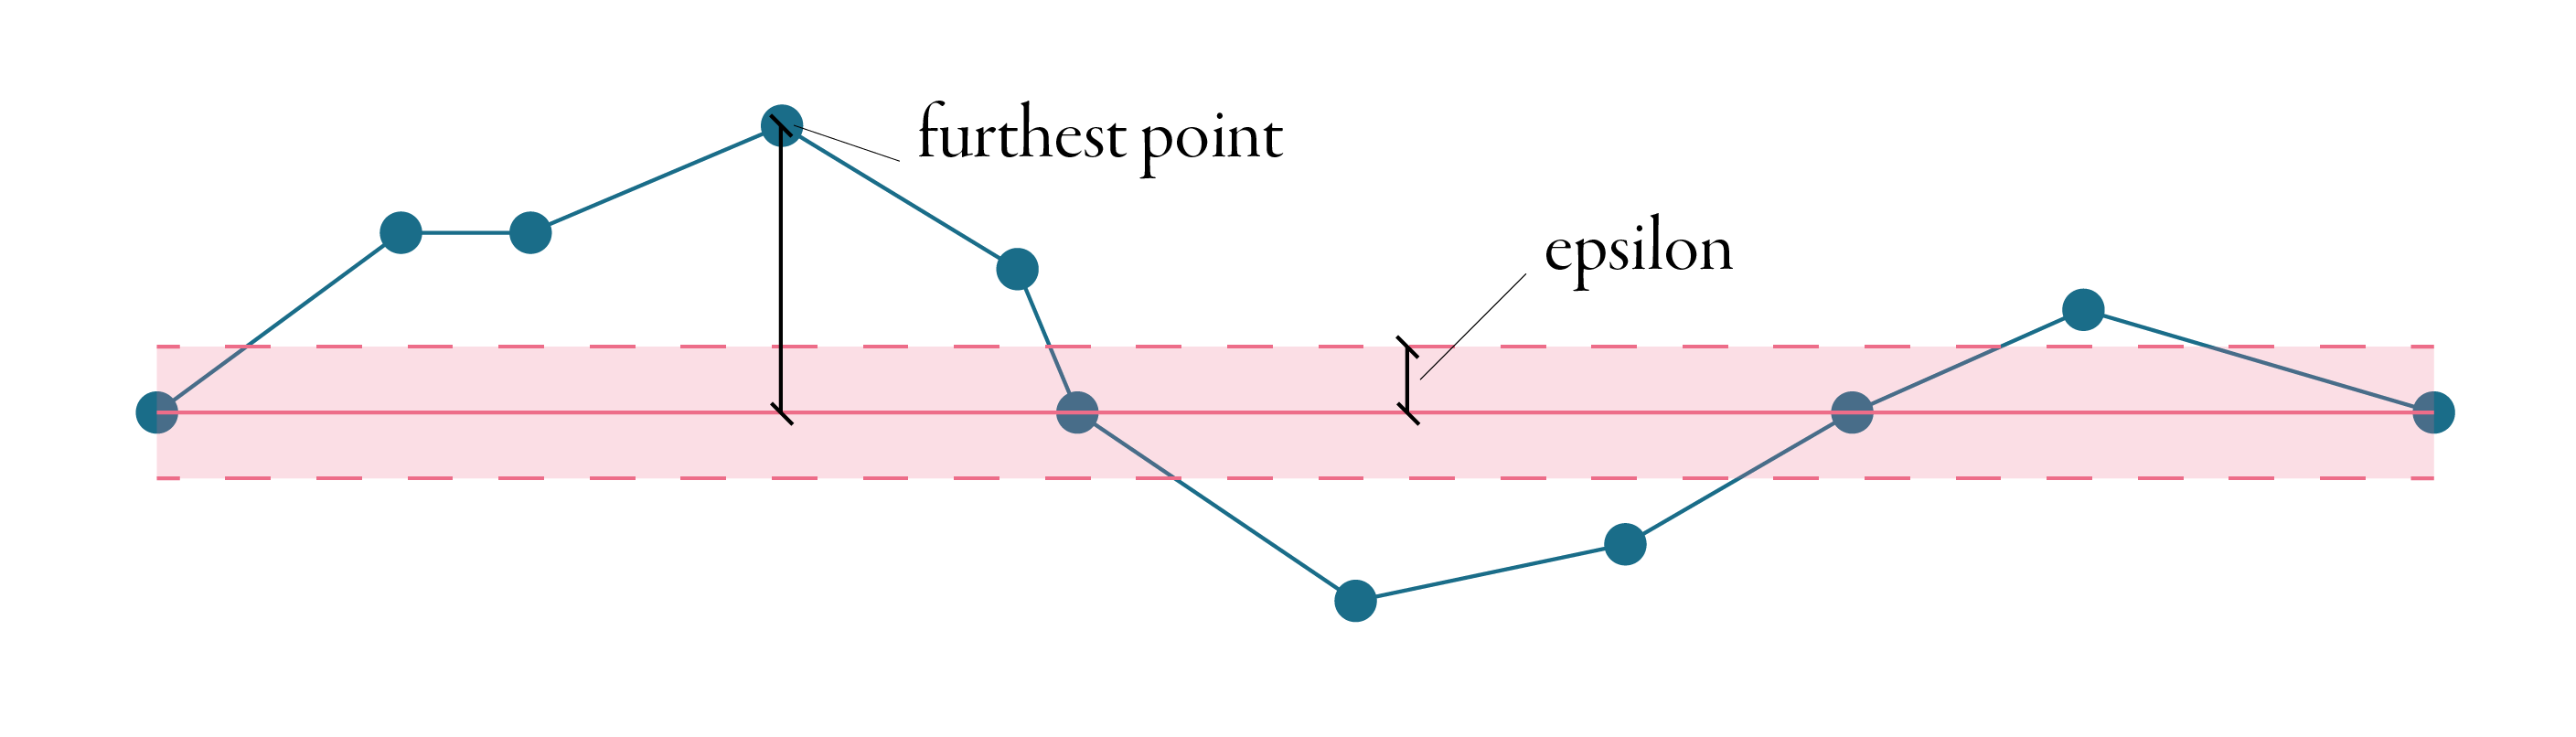
\includegraphics[width=0.45\textwidth]{line_simplification.png}
  \caption{Ramer-Douglas-Peucker Line Simplification}
\end{figure}

We compared the results of our preprocessing with the original Quick, Draw! data to verify we were following the process correctly. We passed in the raw Quick, Draw! data to our function and compared its output with the corresponding sketch in the simplified dataset. Below are some examples of the simplified images:

\begin{figure}[H]
  \centering
  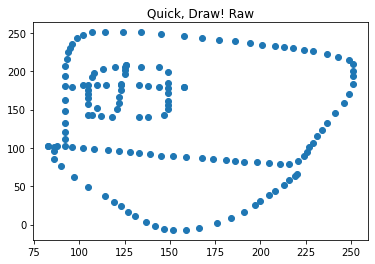
\includegraphics[width=0.45\textwidth]{quickdraw_raw_house.png}
  \caption{Quick, Draw! Raw Data of a House}
\end{figure}

\begin{figure}[H]
  \centering
  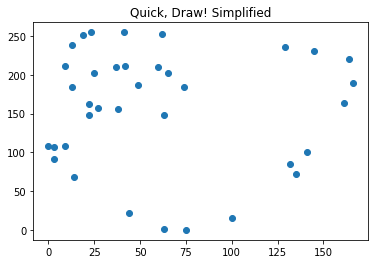
\includegraphics[width=0.45\textwidth]{quickdraw_simplified_house.png}
  \caption{Quick, Draw! Preprocessed Data of a House}
\end{figure}

\begin{figure}[H]
  \centering
  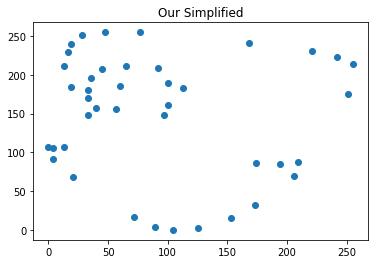
\includegraphics[width=0.45\textwidth]{our_simplified_house.png}
  \caption{Our Preprocessed Data of a House}
\end{figure}

As seen in the plots, our simplified data was not identical to the data provided by Quick, Draw!, as there are more points remaining in some areas and the scale is larger, but we found that this did not affect our model’s ability to predict on our sketches accurately. 

%--------------------------------------------------------------------------
\subsection{Models for Classification}

The model we used was architected by the Google TensorFlow team and is described as an RNN-based recognizer \cite{tensorflow-architecture}. The model is a CNN Long Short-Term Memory (LSTM) architecture which is common for image classification. This model involves taking a drawing encoded with stroke data, applying 1-dimensional convolutions to the image, running the image through LSTM layers, and passing the sum through the softmax function. Then, the output of the softmax function is used to predict the most likely class of the image. Below, we can see a diagram depicting how the model works, end-to-end.

\begin{figure}[H]
  \centering
  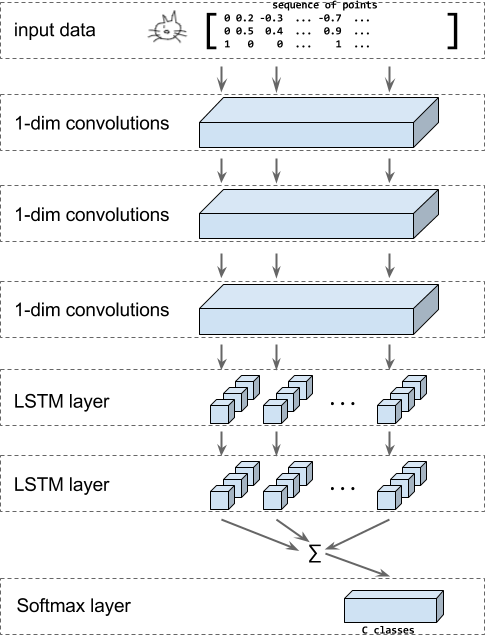
\includegraphics[width=0.45\textwidth]{quickdraw_architecture.png}
  \caption{RNN-Based Model Architecture}
\end{figure}

%--------------------------------------------------------------------------
\subsection{Sketch Generation with GANs}

The original roadmap for this project was to first create a model that can classify sketches, in which a human player can provide a sketch and the computer can return a prediction. We then wanted to flip the roles such that the computer will generate a sketch that the human player can guess. The approach for implementing the latter is to utilize GANs. A GAN, or Generative Adversarial Network, utilizes two models – a generator and a discriminator – that will compete against each other. The purpose of the generator is to generate an image starting from random noise such that it can fool the discriminator. The task of the discriminator is to successfully identify if an image is either produced by the generator or is from the training set.

The plan for implementing the GAN involves the following steps:
\begin{enumerate}
  \item Generate an image of any kind – we used MNIST as it is a simple and commonly used dataset. 
  \item Apply this for a single stroke of a particular set of sketches from the Quick, Draw! dataset
  \item Retrain the model for subsequent strokes.
\end{enumerate}

The idea was that the individual trained then re-trained GANs will be able to produce a set of strokes that can combine into a sketch. We hoped that under the rules of pictionary, the generator would provide a challenging but identifiable sketch for the human player.

%--------------------------------------------------------------------------
\section{Results}

In this section we will discuss the results we found both analytically and empirically. We compute the model’s accuracy on easy and hard images and subjectively assess the model’s quality through a playable game.

%--------------------------------------------------------------------------
\subsection{Accuracy}

\begin{figure}[H]
  \centering
  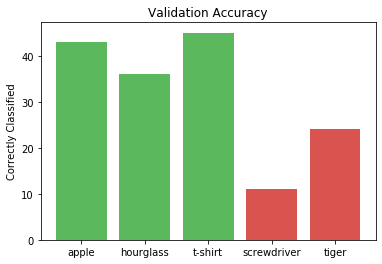
\includegraphics[width=0.45\textwidth]{accuracy.png}
  \caption{Classification Accuracy Chart}
\end{figure}

The chart above displays our model’s accuracy on the Quick, Draw! training data across five different categories. The y-axis represents how many sketches were correctly classified, out of a total of 50 for each category. We can see that apples, hourglasses, and t-shirts all had over 60\% of sketches classified correctly, as these are relatively simple objects that do not leave much room for interpretation. Contrarily, screwdrivers and tigers had accuracies below 50\%. These are two examples of sketches that likely contain many strokes, and can be drawn from several perspectives, so the training images could appear vastly different

%--------------------------------------------------------------------------
\subsection{Examples}

We implemented our model into a playable version of Pictionary involving a user and our neural network. Once the user has drawn an image, the computer attempts to predict what they’ve drawn. Below are some examples of user-drawn images and the class predicted by the computer along with the confidence of each prediction.

\begin{figure}[H]
  \centering
  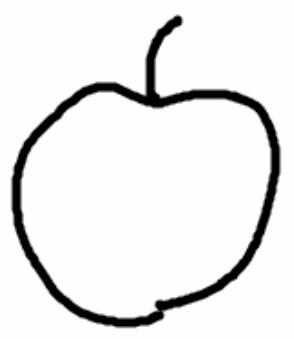
\includegraphics[width=0.15\textwidth]{apple_drawing.png}
  \caption{Apple with 81.78\% Confidence}
\end{figure}

\begin{figure}[H]
  \centering
  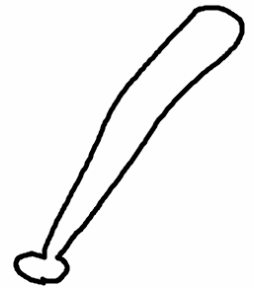
\includegraphics[width=0.2\textwidth]{bat_drawing.png}
  \caption{Baseball Bat with 88.33\% Confidence}
\end{figure}

\begin{figure}[H]
  \centering
  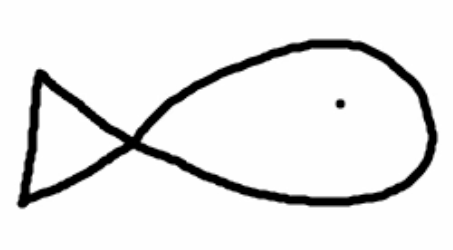
\includegraphics[width=0.25\textwidth]{fish_drawing.png}
  \caption{Fish with 96.85\% Confidence}
\end{figure}

\begin{figure}[H]
  \centering
  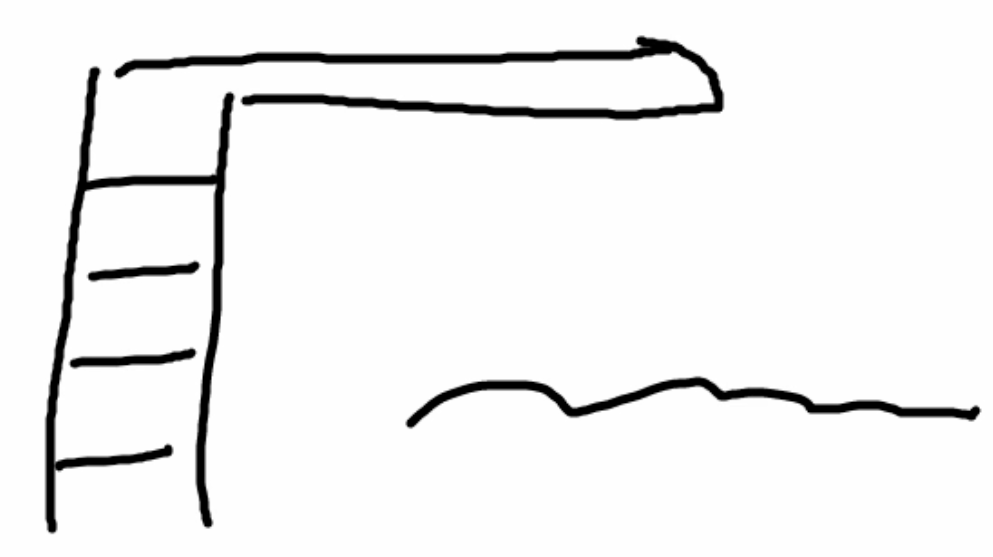
\includegraphics[width=0.35\textwidth]{diving_drawing.png}
  \caption{Diving Board with 76.61\% Confidence}
\end{figure}

Below is our GAN’s sketch of an envelope:

\begin{figure}[H]
  \centering
  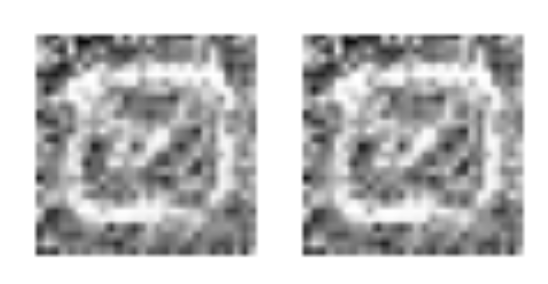
\includegraphics[width=0.4\textwidth]{gan_sketch.png}
  \caption{Envelopes Sketched by a GAN}
\end{figure}

We faced many challenges while attempting sketch generation, which are discussed in the following section.

%--------------------------------------------------------------------------
\section{Analysis}

While experimenting, we noticed the model performed poorly on some objects due to variation in the training data. We also ran into many issues while implementing GANs, mainly because of how inconsistent the training data is since artists can have different stroke orders while drawing the same object. The GANs also often ran into mode collapse issues, which is discussed in further detail below.

%--------------------------------------------------------------------------
\subsection{Issues}

We discovered that the training set had some inconsistencies. One of the key attributes of sketches is that artists interpret objects differently, leading to variations between sketches. For example, words like ``bat'' can be interpreted in the context of baseball or animals. Homonyms like this cause variance in the training data. Also, objects such as a ``car'' can be drawn from different angles such as a top view or side view, creating additional variance. These issues affect the model’s robustness significantly.

While attempting to implement sketch generation, we ran into several issues. The GANs were easily able to generate the images from the MNIST dataset, however when we tried to train the model on even a single stroke, the generator failed to generate an identifiable stroke. Normally for GANs, the output of the generator should produce images that are slightly different in an attempt to fool the discriminator. However, sometimes the generator is only able to produce one image or a very small set of images. This can be attributed to the generator finding a small set of images that can easily fool the discriminator. 

On the other hand, when a generator is only able to produce a small set of images, the discriminator is trapped into finding the solution that predicts for those images. This keeps repeating itself where every generation of generator and discriminator is specifically targeting and optimizing for the previous generation. This results in the GAN producing a repeating set of images that have little resemblance to the wanted target. This is called mode collapse and is a common problem for GANs, and is an active area of research.

%--------------------------------------------------------------------------
\section{Conclusion and Future Work}

Through this project, we saw firsthand the differences in image and sketch recognition, and how the latter can pose interesting challenges. Even with the sparse representations we had of our sketches following preprocessing, the neural network was powerful enough to recognize most sketches, even some that other humans might not be able to identify.

Future work in this area could focus on pursuing the concept of sketch generation further and attempting to resolve the issues we faced. If able to produce computer-generated sketches, we could expand upon the game we created and have a two-way Pictionary interface.

{\small
  \bibliographystyle{ieee_fullname}
  \bibliography{pictionary}
}

\end{document}
